% glossary.tex - thesis example with glossary
\documentclass[12pt,glossary]{dalthesis}
% to prepare draft version use option draft:
%\documentclass[12pt,draft]{dalthesis}


\usepackage{amssymb}
\usepackage{blindtext}
\usepackage{enumitem}
\usepackage[utf8]{inputenc}
\usepackage[english]{babel}
\usepackage{amsthm}
\usepackage{graphicx} %package to manage images
\graphicspath{ {Figures/} }
\usepackage[linesnumbered,ruled]{algorithm2e}
\usepackage{multirow}
\usepackage{setspace}

\renewcommand{\baselinestretch}{2.0}

\newtheorem{theorem}{Theorem}[section]
\newtheorem{corollary}{Corollary}[theorem]
\newtheorem{lemma}[theorem]{Lemma}


\begin{document}

\macs  % options are \mcs, \macs, \mec, \mhi, \phd, and \bcshon
\title{COMPACT REPRESENTATION OF SEPARABLE GRAPH}
\author{Xiang Zhang}
\defenceday{1}
\defencemonth{August}
\defenceyear{2017}
\convocation{May}{2017}

% Use multiple \supervisor commands for co-supervisors.
% Use one \reader command for each reader.

\supervisor{Dr. Meng He}
\reader{D. Odaprof}
\reader{A. External}

\nolistoftables
\nolistoffigures

\frontmatter

\begin{abstract}
This is a test document.
\end{abstract}

\printglossary

\begin{acknowledgements}
My Supervisor, Dr. Meng He, deserves the most praise for his invaluable guidance, friendship and suggestions. I would also like to thank all of the friends and acquaintances I have made at Dalhousie University. They have made this journey something to remember. Without everyone’s support and guidance this project would have not been a success.
\end{acknowledgements}

\mainmatter

\chapter{Introduction}

Nowadays, many applications use graphs to show the relationship and represent connectivity between multiple objects. The usage of such graphs are so popular in representing various of data type including link structure of the web, 3d models in mesh, geographic maps, and surface meshes in computer graphics, etc. As the graphs inevitably grow very huge, the space issue becomes ever more important. Hence, the problem of designing space-efficient data structures to represent graphs while supporting efficient queries operations, has drawn a great deal of attention. 

\bigskip
Plenty of previous works have been conducted to represent graphs "succinctly", which means represent the graphs in a compact representation whose space cost is close to the information-theoretic lower bound, and still supports efficient query operations. The problem of succinctly representation of a graph can be formalized as: given a graph $G = (V, E)$ of type $\chi$, where n and m are numbers of vertexes and edges, respectively, then represent $G$ using $\lg | \chi | + o(\lg | \chi | )$ bits of space, and support a set of query operations on the graph in constant time ( assuming we can access $\Theta(\lg n)$ consecutive bits in one operation ). The space bound may not be satisfied, alternatively, trade-off between space cost and query time can be further investigated.  

\bigskip

A considerable strategy to save the space when represent graphs is taking advantage of structural properties of graphs. In practice, the most common structural property of graphs is they have small separators. A graph has separators if it can be partitioned into two subgraphs in approximately equal size by removing a small amount of vertexes. For example, Planar graphs, have $O(n^{1/2})$ separators, and even graphs that are not strictly planar because of crossings, such power networks, have small separators too. More generally, nearly all graphs that represents connections relationship in low dimensional spaces have small separators. We say a graph is separable if it is taken from a class of graphs that satisfies an $n^{c}$-separator theorem~\cite{separator-theorem} for some constant c $<$ 1.

\bigskip

In this project, we are interested in improving a compact representation mechanism for separable graphs presented by a previous work ~\cite{compact-representation}. In which work the authors proposed an approach to representing separable graphs compactly. Their representation used $O(n)$ bits, meanwhile using constant time on degree or adjacency query, and neighbour listing for one vertex in constant time per neighbour (They took advantage of $O(\lg n)$-bit parallelism computation to access $\Theta(\lg n)$ consecutive bits in one operation). Graphs with good separators got good compression by using their representation, and even graphs that are not strictly separable, their representation still works well because the separable components in those graphs can be compressed.In their paper, they provided detail description for compressing the graph by building two structures: the adjacency table and the root-find structure ~\cite{compact-representation}, which used vertex separators to encode the graph into a shadow adjacency table ~\cite{compact-representation}, as well as support constant time on query operations. But their experiment implemented the data structure by using edge separator instead of vertex separator, which means the shadow label and root-find structure were not needed. In this project, we implement the data structure by using edge separator, and conduct experiment on it.

\bigskip
\bigskip

We firstly follow their idea to implement the data structure by using edge separator. The data structure is building by recursively partitioning a graph into two subgraphs until only one vertex left. During the partition process, an edge separator tree is built. Then make use of the edge separator tree to renumber the vertexes. We store an adjacency list for each vertex, then concatenate the adjacency lists in the order of renumbered vertex to form an adjacency table. Each pair of vertexes in the adjacency is stored by encoding the difference $d$ between the two vertexes, and all the differences are stored contiguously as a sequence of bits in memory. We show, by using adjacency table, $O(n)$ bits are sufficient to encode the separable graph. 

\bigskip
\bigskip

Next, we implement several index structures to support degree and adjacency query in constant time, and neighbour listing in constant time per Neighbour. The index structures contains all the index structures involved in their experiment, as well as two index structures implemented by us which apply succinct data structures on bit vector. In their paper, they encoded the degree of each vertex at the start of each adjacency list. However, the space of degree can be saved in some cases, which causes a trade-off between the time to support degree queries and the space to encode the graph.

\bigskip
\bigskip

We compare the performance of various indexing structure by conduct a DFS on the graph represented by different indexing structure. We also compare our space and time cost to that of an array-based adjacency list.  

\section{Related Works}

There has been considerable works dedicate to compress graphs such as planar graph, k-Page graph and separable graph. The first attempt of succinct representation of graphs was conducted by Jacobson~\cite{Jacobson}, who first showed how to represent planar graph by using O(n) bits while supporting adjacency queries in $O(\log n)$ time. His approach decomposes a planar graph into at most four one-page graph which is represented as a sequence of balanced parentheses. His representation extended naturally to a $k$-page graph problem, where k$\geq$1.

\bigskip
\bigskip

Munro and Raman~\cite{Munro} improved the time for adjacency queries to O(1) time while using $8n+2m$ bits where $n$ and $m$ are numbers of vertexes and edges respectively. Their work gives great reduction in the higher order term for number of bits regarding Jacobson's parenthesis representation, and further expands the types of operations on parenthesis representation. Geary $et$ $al.$~\cite{Geary} gave a conceptually simpler representation compared to Jacobson's data structure, they used $2n+o(n)$ bits while supporting natural parenthesis operations in $O(1)$ time. The space constants on the high order term has been improved by Chuang $et$ $al.$~\cite{Chuang}, and further by Chiang $et$ $al.$~\cite{Chiang}. The former proposed another encoding mechanism based on $canonical orderings$ of a planar graph, then used a $multiple parentheses sequence$ to represent the graph, while the latter generalized the notion of canonical orderings to orderly spanning trees and improved constant factors in terms of numbers of vertexes and edges. 

\bigskip
\bigskip

A succinct representation for a k-page graph when k is large to support various navigational
operations more efficiently, was proposed by Barbay $et$ $al.$~\cite{Barbay}, whose representation used $n+2m\lg n + m \cdot o(\lg k) + o(m)$ bits to support adjacency queries in $O(\lg k \lg \lg k)$ time, degree queries in constant time and neighbourhood in $O(d(x) \lg \lg k)$, where $d(x)$ is the degree of vertex $x$, or used $n+(2+\epsilon)m\lg k + m \cdot o(\lg k) + O(m)$ bits to support adjacency, degree and neighbourhood queries in $O(\lg k)$, $O(1)$ and $O(d(x))$ time, respectively, where $\epsilon$ is any constant satisfies $0< \epsilon <1$.   

\bigskip
\bigskip

Blandford $et$ $al.$~\cite{compact-representation} made use of the unlabelled graphs with small separators to compactly represent the graph, whose representation used $O(n)$ bits on graph satisfies a $n^{c}$-separator theorem, while support degree and adjacency queries in $O(1)$ time, and neighbourhood queries in constant time per neighbour. Subsequently, Blelloch $et$ $al.$~\cite{succinct-representation} proposed a succinct representation on unlabelled separable graphs, which used $lg| \chi |+ o(n)$ bits to represent a graph in type $\chi$, while holding the same time bounds as the performance of Blandford's representation.       

\section{Preliminaries}

\textbf{Graph Separator}. A family of graphs $G$ is define separable if : it is closed under taking subgraphs, and satisfies the $f(.)$-separator theorem ~\cite{separator-theorem} if there is a constant $\alpha$ $<$ 1 and $\beta$ $>$ 0 such that each member graph in G with n vertexes has a separator set S of size $|S|$ $<$ $\beta f(n)$, that partition the graph into two parts A and B, with at most $\alpha n$ vertexes in each. A graph is separable if it belongs to a separable family of graphs. 

\bigskip
\bigskip

In this project we focus on the graphs that satisfy the $n^{c}$-separator theorem for some constant $c < 1$. One class of graphs that reach this specifications is the planar graphs, which satisfies the theorem that $c = \frac{1}{2}$ . Another example can be well-shaped meshes in $\mathbb{R}^{d}$ , with separators of size $O(n^{1-1/d})$~\cite{ separators-sphere-packing}.

\bigskip
\bigskip

Lipton $et al$.~\cite{Nested-Dissection} prove that all classes of graph which satisfy $n/(\log n )^{1+\epsilon}$-separator theorem have bounded density. The bounded density means that every n-vertex member in a class if graphs has bounded $O(n)$ edges. So we can assert that the separable graphs have bounded density.

\bigskip
\bigskip

By making use of the definitions above, we define a class of graphs G satisfies a $f(n)$-edge separator theorem if there are constant variables $\alpha$ $<$ 1 and $\beta$ $>$ 0 such that each member graph in $G$ with n vertexes, has an edge separator with at most $\beta f(n)$ edges whose removal partitions the graph into two subgraphs with at most $\alpha n$ vertexes in each. The edge separator is not as common as the vertex separator, because a graph with an edge separator of size s also has a vertex separator of size s at most, but no similar bounds holds when it is conversed~\cite{compact-representation}.

\bigskip
\bigskip

In this project, we will only consider the connected graph, which means all vertexes in the graph have nonzero degree, and we assume each step of partitioning always returns a edge separator set of size $O(n^{c})$.

\bigskip
\bigskip

\textbf{Queries}. Our data structure supports three kinds of queries on separable graphs: adjacency queries, degree queries and neighbour listing. The adjacency query checks whether there is an edge between two vertices, the neighbour listing returns the neighbours of a given vertex, and the degree query reports the number of edges connected to a given vertex.

\bigskip
\bigskip

\textbf{Bit Vector}. The compact representation stores a separable graph as difference-encoded bit sequence in memory. To support the three kinds queries (adjacency queries, degree queries and neighbour listing) in constant time, knowing both the number of encoded adjacency lists in the sequence up to an index position, and the start position of a particular adjacency is necessary. More formally, the compact representation requires data structures that support rank and select operations in constant time: Given a set $B[0...n)$ to represented a subset $S$ of a universe $U = [0...n)$ = $\{0,1,...,n-1 \}$, where $B[i] = 1 \ iff \ i \in S$,

\begin{itemize}[noitemsep]
\item $rank_{q}(x)$ = $\{k \in [0...x] : B|k| = q \}$
\item $select_{q}(x)$ = $ min \{ k \in [0...n) : rank_{q}(k) = x \} $ 
\end{itemize}

\bigskip

In this project, we use two kinds of succinct data structure on bit vector : RRR~\cite{RRR} and SD vector~\cite{SD-vector}, to build the index structure which supports queries on separable graph. Both structures satisfy information-theoretic lower bound, and still supports efficient rank and select query operations.

\bigskip
\bigskip

\textbf{Adjacency Tables}. An adjacency list representation for a graph associates each vertex in the graph with the collection of its neighboring vertices. For use as a data structure, the main alternative to the adjacency list is the adjacency matrix. For a sparse graph (most pairs of vertices are not connected by edges), in our case, a graph has $bounded \ mdensity$, an adjacency list representation is significantly more space-efficient than an adjacency matrix representation: the space cost of the adjacency list representation depends on the number of edges and vertices in the graph, while the adjacency matrix representation is stored as the square of the number of vertices. Generally, an adjacency list representation for an undirected graph requires 8$|E|$ bytes (2(32)$|E|$ bits) of space, where $|E|$ is the number of edges in the graph. However, it is not space-efficient enough yet.

\bigskip
\bigskip

In our project, we assign each vertex in the graph an integer label. For each vertex, we store an adjacency list which contains its all neighbouring vertexes. If a vertex with label $v$ has neighbours $v_{1}, v_{2}, v_{3}, ...,v_{n}$ in ascending sorted order, then we encode the difference between each adjacency pair in the adjacency list as $|v_{1}-v|, \ |v_{2}-v_{1}|,\  |v_{3}-v_{2}|,\ ...,\ |v_{n}-v_{n-1}|$ contiguously, which forms a sequence of bits stored in memory. We use the gammacode~\cite{Gamma} to encode the differences, which uses $2\lfloor \log n \rfloor + 1$ bits to encode a difference. The difference $v_{1} - v$ may be negative in some cases, we here store a one-bit flag that value. To implement one of our index structures, the degree of each vertex needs to be encoded at start position of the corresponding adjacency, but in other circumstances the space of degree can be saved. By concatenating all the adjacency lists in the order of the vertex labels, we form an adjacency table. To access the adjacency list of a vertex, knowing the starting position of the adjacency
is necessary. The easiest and fastest approach is to store an array of offset pointers of size $O(\log (n))$ for each. But if doing so, we would use $nO(\log (n))$ space, which exceeds our space bound. Alternatively, we implement other two index structures proposed by Blandfor~\cite{compact-representation}, as well as two index structures based on succinct data structure on bit vector, which use less space cost down to $O(n)$ bits.
\bigskip
\begin{lemma}
An adjacency table can support degree queries in $O(1)$ time, and neighbour
listing in $O(d)$ time, where $d$ is the degree of the vertex.
\end{lemma}
\bigskip 
\begin{proof}
To access an adjacency list of a particular vertex, we use our index structure to locate its starting position in constant time. Each adjacency list consists of a encoded degree number and a sequence of encoded differences, which use $O(\log (n))$ bits and $dO(\log (n))$ bits respectively. By taking advantages of the $O(\log n)$-bits parallelism computation, we can decode any $O(\log (n))$-bits value in constant time, like using lookup table. Hence we can decode the degree at the starting of each adjacency list in constant time. For neighbour listing, we decode each difference pair in constant time. So it takes constant time to make degree queries, and $O(d)$ time to make neighbourhood queries, where d is the degree of the vertex.
\end{proof}

\section{Outline}
This report is organized as follows. Chapter 1 shows the motivation of this project, and provides some preliminaries used in this project. Chapter 2 and 3 explain the construction and usage of the edge separator tree and several index structures respectively. Chapter 4 describes the experiment setup and examines the performance of our data structure. Chapter 5 shows the conclusion as well as the future work of our project.

\chapter{Edge Separator Tree}

To compactly represent the tree, the first thing we need to do is building an edge separator tree from the original tree. The tree-building process is based on recursively partition the tree into two parts using edge separator. One example that illustrates the function of edge separator is shown in Figure 2.1: assuming we have an 8-vertex graph $G_{1}$ with 9 edges, by removing the two edges $(v_{1}, v_{9})$ and $(v_{1}, v_{5})$, we can partition $G_{1}$ into two parts with 4 vertexes in each. Hence the edge separator in this partitioning step is $\{(v_{1}, v_{9}),(v_{1}, v_{5}) \}$.

\bigskip

\begin{figure}[ht]
\centering
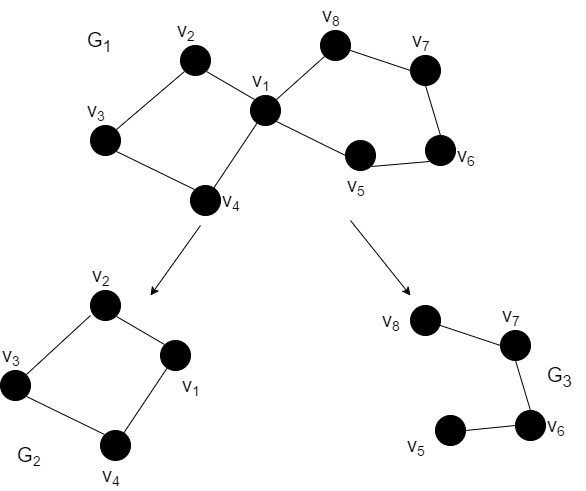
\includegraphics[width=0.7\textwidth]{partition}
\caption{An example of a partition process using edge separator}
\end{figure}

\bigskip

We can see that each time we make a partitioning on a graph, it splits its vertex set and parts of edges set, and removes some edges. if we perform this partitioning recursively until only one vertex left, then we have an edge separator tree from the graph, one edge separator tree for the $G1$ in Figure 2.1 is shown in Figure 2.2. Each vertex in a graph will appear once in a leaf of the edge separator tree build from that graph. Each internal node is the set of edges used as edge separators to make partitioning in each step.

\begin{figure}[ht]
\centering
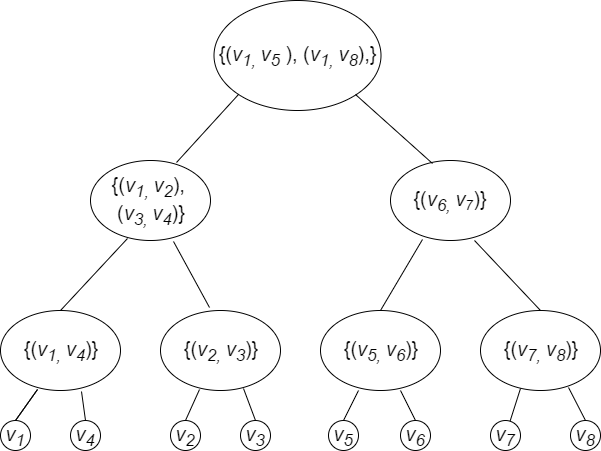
\includegraphics[width=0.8\textwidth]{separatorTree}
\caption{An example of edge separator tree}
\end{figure}

\bigskip
\bigskip
Note that we arbitrarily decide which side of partition will be the left child or the right child in this stage. The tree is also not perfect balanced in some cases (e.g. one child is a leaf and the other is an internal node), the side of the children is also decided arbitrarily. We will take advantages of this "freedom" to further reduce the space to encode the graph in later time. The vertex labels may be disordered by making in-order traversal on the edge separator tree (e.g. in Figure 2.2 the order of the vertexes after in-order traversal is :$v_{1}$, $v_{4}$, $v_{2}$, $v_{3}$, $v_{5}$, $v_{6}$, $v_{7}$, $v_{8}$), we will renumber these vertex by making a in-order traversal along the edge separator tree.

\bigskip
\bigskip

\textbf{METIS Partition Library}. To recursively partition the graph, we use METIS's API in our project. METIS is an open source library developed by Karypis lib in University of Minnesota. It supports set of serial programs for partitioning graphs and partitioning finite element meshes. The algorithms implemented in METIS are based on the multilevel recursive-bisection, multilevel k-way, and multi-constraint partitioning schemes [2]. The METIS partitioning API returns one integer list with vertex index as key, and a flag 0 or 1 to indicate which side of partitioning the vertex belongs to. The returned value of METIS API does not provide information about edges, and the API takes two integer arrays (adjacency list of current graph and the index of vertex in adjacency list)as input parameters, hence before each calling of the METIS API, we need to generate an adjacency list and an index list for the current graph to be partitioned, and in order to collect the edge separators, we need both the adjacency list and the returned values after calling the API.

\bigskip
\bigskip

The Algorithm to build the separator tree is given in Algorithm 1. Here we use $(V,E)$
to represent a graph for simplicity, but in fact the METIS API takes formalized adjacency list and the index list as input parameters. So each time to call the METIS API, the current vertex set need to be renumbered temporally in contiguous ascending numbers, and the adjacency list needs to be initialized according to the temporally order. The METIS API also does not support to partition the graph with the vertex amount under 3, hence the very basic partitioning cases are defined by ourself.

\bigskip

\begin{algorithm}
    \underline{buildTree} $(V,E)$\;
    \eIf{$|V|=1$}
      {
        return $V$\;
      }
      {
      	$(V_{a},V_{b})$ $\leftarrow$ \textbf{METIS$\_$API} $(V,E)$  \;
		$E_{sep}$ $\leftarrow$ \textbf{findEdgeSeparator} $(V,E,V_{a},V_{b})$ \;
		$E'$ = $E \  - \ E_{sep}$   \;
      	$E_{a}$ $\leftarrow$ $\{ (u,v) \in E' \ | \  u\in V_{a} \vee v \in V_{b} \}$ \;
		$E_{b}$ = $E'$ - $E_{a}$ \;
		$T_{a}$ $\leftarrow$ \textbf{buildTree} $(V_{a},E_{a})$ \;
		$T_{b}$ $\leftarrow$ \textbf{buildTree} $(V_{b},E_{b})$ \;  
        return \textbf{separatorTree} $(T_{a}, E_{sep}, T_{b})$ \; 
      }
    \caption{Building the edge separator tree}
\end{algorithm}
\bigskip

\textbf{Building Adjacency Table}. After getting the edge separator tree, we need to renumber the vertexes based on an in-order traversal along the tree. Each vertex appears in one leaf of the tree will receive a new label which increases by one when visiting a new leaf node. A mapping table is also generated after completing the traversal, which will be used to build an adjacency list for each renumbered vertex by using the new vertex labels. Then we can build an adjacency list for each vertex, the list contains all the neighbouring vertexes in sorted order. We use gamma code to encode the difference of each adjacency pair in the list (e.g. $v_{1} - v$, $v_{2} - v_{1}$,..., $v_{n-1} - v_{n-2}$), each difference d costs $2\lfloor \log n \rfloor + 1$ bits to be encoded. Note that the value $v -v_{1}$ might be negative, so we store one flag bit for it. We also encode the number of the entries in an adjacency list at the starting position of the list, which will be used to support degree queries in constant time.

\bigskip
\begin{lemma}
Any n-vertex member in a class of graphs which satisfies a $n^{c}-edge$ separator
theorem, can be encoded in $O(n)$ bits using an adjacency table.
\end{lemma}
\bigskip 

\begin{proof}
For each edge $(u, v)$ in an edge separator in a graph with s vertexes, the difference
between vertex u and vertex v is $O(s)$. We use gamma code to encode the difference which would use $O(\log (s))$ bits, so that edge will contribute $O(\log (s))$ bits to the adjacency lists of both vertex u and vertex v. Hence, we charge $O(\log (s))$ to every edge in a separator of a graph with s vertices. Recall that by using the $n^{c}- edge$ separator theorem, each member with n vertexes in the class of the graph has a $\beta n^{c}$ edge separator whose removal partitions the member into two parts with at most $\beta n$ vertexes in each. Let define $S(n)$ to be an upper bound of required bits to encode a graph with n vertexes, and let $\alpha < a < 1 - \alpha $, then $S(n)$ satisfies the recurrence:
\[ S(n) \leq S(an) + S(n-an) + O(n^{c} \log n) \]
This recurrence can be solved to $S(n) = O(n)$, and the bits to encode the degree of all the vertexes is bounded by $O(n)$, because there are $O(n)$ edges in total. So the total space is $O(n)$ bits.
\end{proof}

\bigskip
\bigskip

\textbf{Child-flipping}. When encoding the graph, We contiguously encode the difference between each adjacency pair in the list by using gamma code. The gamma code use $2\lfloor \log n \rfloor + 1$ bits to encode a difference d. If we can make each difference "smaller", in other words, if we can make the labels of vertexes in an adjacency list closer to each other, then we can reduce the space to encode the adjacency list. We arbitrarily decide the side of partitioning during the construction of the separator tree (in our project, we decide the side of partitioning according to the output value of METIS API: '0' to the left child and '1' to right child), so there is a degree of freedom in the way to build the tree. To take advantage of this freedom, we can apply a heuristic optimization method called "child-flipping"~\cite{compact-representation} to our edge separator tree.

The child-flipping algorithm works when making traversal along a separator tree, it tracks the nodes containing vertex labels which appear before and after the vertex labels in the current node. Let define $N_{L}$ to be the left children of current node's left ancestors and $N_{R}$ to be the right children of the current node's right ancestors, $N_{1}$ and $N_{2}$ represents the current node's left child and right child, respectively, and $E_{AB}$ indicates the number of edges between the vertexes in node A and node B. For each node, the vertexes in $N_{1}$ of the current node will have labels less than the vertexes' under the node, the vertexes in $N_{2}$ will have larger labels than all the vertexes under the node, and there is no intersection between the vertexes in $N_{L}$ and $N_{R}$ of the node. The child-flipping exams $E_{N_{L}N_{1}}$, $E_{N_{2}N_{R}}$, $E_{N_{L}N_{2}}$ and $E_{N_{1}N_{R}}$ of each node to ensure that $E_{N_{L}N_{1}} + E_{N_{L}N_{1}} \leq E_{N_{L}N_{1}} + E_{N_{L}N_{1}}$. If not, the child-flipping algorithm swaps the two children of current node. The meaning of making this swap is : after renumbering the vertexes based on an in-order traversal, if $E_{N_{L}N_{1}} + E_{N_{L}N_{1}} < E_{N_{L}N_{1}} + E_{N_{L}N_{1}}$, then the space to encode the edges $N_{L}N_{2}$ and $N_{1}N_{R}$ is greater than that to encode $N_{L}N_{2}$ and $N_{1}N_{R}$, because the difference $v_{N_{2}} -v_{N_{L}}$ is obviously greater than $v_{N_{1}} - v_{N_{L}}$, similar fact works on the difference of $v_{N_{R}}-v_{N_{1}} \  and \  v_{N_{R}}-v_{N_{2}}$.

\bigskip
\bigskip

This heuristic algorithm can be applied to any edge separator tree as a postprocessing
step. However, this process is quite time-consuming, the time cost of applying both METIS and child-flipping in Blandfor $et al.$ ~\cite{compact-representation}'s experiment shows a demonstration on this. To get the four numbers of edges($E_{N_{L}N_{1}}$, $E_{N_{2}N_{R}}$, $E_{N_{L}N_{2}}$ and $E_{N_{1}N_{R}}$ ), we need to have the four vertex sets: $N_{L}$, $N_{R}$, $N_{1}$ and $N_{2}$ for each tree node. The $N_{L}$ and $N_{R}$ of each node in separator tree can be pre-collected, but the $N_{1}$ and $N_{2}$ need to be calculate locally when reach the node. In our project, we make some efforts to reduce the time to conduct this child-flipping processing: Let assume we have a node $N_{a}$ in a separator tree with left child as $N_{b}$ and right child as $N_{c}$, if we knew the $N_{1}$ and $N_{2}$ of Na (denote as $N_{1a}$ and $N_{2a}$), then

\begin{itemize}[noitemsep]
\item for node b : $ N_{1b} = N_{1a}, N_{2b} = N_{2a} \cup N_{Ra}$
\item for node c : $ N_{1c} = N_{1a} \cup N_{La}, N_{2c} = N_{2a}$ 
\end{itemize}

Having this general case, then we can generate the $N_{1}$ and $N_{2}$ for each node during the child-flipping traversal via DFS. The $N_{L}$ and $N_{R}$ of each node in separator tree can be pre-collected via a post-order traversal along the edge separator tree, the vertex set of a node is formed by merging the two vertex sets of its children in sorted order. When needing to expand the current $N_{1}$ or $N_{1}$, we include the new coming $N_{L}$ or $N_{R}$ as distinct sorted set instead of merging $N_{L}$ into $N_{1}$ or $N_{R}$ into $N_{2}$. Note that in term of a node, the size of $N_{L}$ or $N_{R}$ is always smaller that the size of $N_{1}$ or $N_{2}$, respectively. We check an existing of an edge by performing binary on larger sorted set, all of above approaches improve the speed of child-flipping processing significantly .

\chapter{Index Structure}

We already introduce how to encode a graph with good edge separator into difference adjacency table bounded by $O(n)$ bits, but to access to the particular adjacency list for a particular vertex, we need to know the exact starting position in the bit sequence. Hence our representation requires a data structure that support efficient select operations on the bit sequence. Note that, the space cost of the data structure should not exceed our space bound which is $O(n)$. Blandfor $et al.$ has proposed three kinds of index structure: $direct$, $semi-direct$, and $indirect$~\cite{compact-representation} to support efficient select queries. In addition to these three structures, we also implement other two index structures based on RRR and SD Vector respectively, we will henceforth call these two RRR-based and SDV-based index structure. 

\bigskip
\bigskip

\textbf{Direct indexing structure}. The easiest way to access to the starting position of 
any adjacency list is to store an offset pointer for each vertex. Because our representation uses $O(n)$ bits to store a separable graph, one offset pointer will use $\Theta (\log (n))$ bits. For all vertexes, it will use $n \Theta (\log (n))$ in total. If we want to locate the starting position of any vertex, only one memory access is needed, so this approach is fastest among the five index structures. In our implementation, we allocate one word (32 bits) space for each vertex, hence the total space for this direct index structure is 4$n$ bytes.

\bigskip
\bigskip

\textbf{Semi-direct indexing structure}. This $semi-direct$ index structure is very similar to the $direct$ structure, but instead of allocating one word space for each vertex, we use two words to store four offset values. Let say we have four vertexes $v_{n}$, $v_{n+1}$, $v_{n+2}$, $v_{n+3}$, The first word space will store the pointer value of $v_{n}$, then use the second word to store three offset value $v_{n+1}$-$v_{n}$, $v_{n+2}$-$v_{n}$, $v_{n+3}$-$v_{n}$. If the space of the three offset values exceeds one-word bound, then store the offsets somewhere else, then the second word store a pointer pointed to them. Compared to the $direct$ structure, if the vertex satisfies $v_{id}$ mod 4 = 0, then it works exactly as same as $direct$ structure, if not, it firstly gets the real offset by adding the corresponding offset to the first pointer value, then access the memory directly. If every four vertexes fit into two-word space, then this $semi-direct$ structure would use half of the space used by $direct$ structure.      

\bigskip
\bigskip

\textbf{Indirect indexing structure}. Note that the above two index structure use $n \theta (n)$, which exceeds $O(n)$ space bound. To limit the space cost within the bound, Blandfor $et al.$ implement the third structure : $indirct$, which use $O(n)$ space meanwhile supports constant time on locating vertex. The component of the structure is shown in  Figure 3.1: we firstly divide all vertexes into blocks with $\log(n)$ vertexes in each, then we further divide each block into subblocks. Each subblock contains a minimal number of vertexes whose indexing offset length reaches at least $k\log(n)$ bits for some constant number $k$. We store a bit vector with $\log(n)$ bits length for each block, if $v_{i}$ is the first vertex in its subblock, then the ($i$ mod $\log (n)$)$_{th}$ bit in the vector of its block is set to 1, otherwise 0. We only store the offset pointers of vertexes if their corresponding bits in bit vector are 1. This will require $O(n)$ bits in total.  

\bigskip

\begin{figure}[ht]
\centering
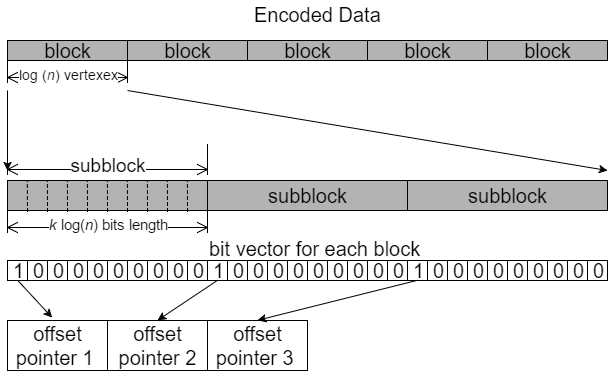
\includegraphics[width=1.0\textwidth]{indirect}
\caption{The architecture of the $indirect$ index structure}
\end{figure}

\bigskip

To locate the starting position of a particular vertex, we firstly find which block the vertex is in by dividing the vertex label with $\log(n)$ (number of vertexes in each block). Next we check the bit vector of that block to find which subblock contains the vertex. Since we store the offset pointer for each vertex which is the first one in its subblock, we can know the starting position of the target subblock, then we decode the subblock. Although we will get all the adjacency lists within the subblock if do so, the degree information of each vertex is also encoded, hence we can have the adjacency list of the target vertex easily. The bit vector of each block has $\log(n)$ bits, each subblock is $k\log(n)$ bits long, determining and decoding the subblock can be completed by using lookup table, which uses constant time to check $\Theta(\log(n))$ bits.         

\bigskip
\bigskip

\textbf{RRR-based indexing structure}. RRR is a succinct data structure which was first proposed by Raman $et al$.~\cite{RRR}. This data structure works on bit sequence $S[0,...,n)$ in such a way that provides rank and select operations in $O(1)$ time at the price of $nH_{0}(S)+o(n)$ space cost, where $H_{0}(S)$ is the empirical zero-order entropy of the sequence. The RRR data structure divides the original bit sequence into several superblocks, then divide the superblocks further. For each block it stores a number to indicate the number of ones or zeros in the block. The number would be used as a lookup key in a table. Besides that, it also stores an offset which indicates which of the blocks the number is in. Offset is also used as an index in the table. By grouping blocks into superblock, RRR can avoid iterating over each block to conduct a rank or select query.

\bigskip
\bigskip

RRR efficiently compresses a bit set if the set is very sparse populated, we take advantage of this feature of RRR and implement a indexing structure based on it. The original graph is encoded into a bit sequence by using gamma code, and we know the length of this sequence. Hence we can maintain another bit set with same length as the encoded bit sequence, in which we set a bit to '1' if it is the starting point of an adjacency list, otherwise we set the bit to 0. By doing so, we get a bit set which is very '1' sparse, then we can build RRR bit vector on this bit set. To locate a particular vertex, we only need to conduct a $select$ query on the RRR bit vector, and we will know its starting position in the encoded bit sequence in constant time. Since the encoded bit sequence is $O(n)$ bits long, and for a n-bit sequence, RRR needs $nH_{0}(S)+o(n)$ bits to support constant $rank$ and $select$ queries. We do not need to store additional information besides RRR structure, so the space cost will not exceed our bound. 

\bigskip
\bigskip

\textbf{SD Vector-based indexing structure}. SD Vector is a bit vector that can compress very sparse populated bit vectors by representing the positions of 1 by the Elias~\cite{Elias}-Fano~\cite{Fano} representation for non-decreasing sequences. Given a bit set $B[0,...n-1)$ with $m$ ones ($m << n$),   the SD Vector uses $m \log n/m  + 2m + o(m)$~\cite{Practical-Entropy} bits to store the bit set, meanwhile support constant time $rank$ and $select$ queries. The idea of SD Vector-based indexing structure is very similar to RRR-based indexing structure. We firstly maintain a bit sequence which has the same length as the encoded graph bit sequence, next we mark the bits which indicate the starting position of an adjacency list, then we build the SD Vector on this bit sequence. In order to locate the starting position of a particular vertex, we use this SD Vector to perform a $select$ operation. 


\chapter{Experiment}


\begin{table}[ht]
\centering
\caption{Graph List}
\label{graph-list}
\begin{tabular}{|l||c|c|c|c|}
\hline
\multicolumn{1}{|c||}{Graph} & Vertexes & Edges   & Max Degree & Source        \\ \hline
feocean                   & 143437   & 409593  & 6          & 3D mesh       \\
m14b                      & 214765   & 1679018 & 40         & 3D mesh       \\
febody                    & 45087    & 163734  & 28         & Scotch Graphs \\ 
wave                      & 156317   & 1059331 & 44         & RIACS Grids   \\
558a                      & 110971   & 741934  & 26         & Cytoscape     \\
144                       & 144649   & 1074393 & 26         & Cytoscape     \\
bcsstk30                  & 28924    & 1007284 & 218        & Matrix: HB    \\
bcsstk31                  & 35588    & 572914  & 188        & Matrix: HB    \\ \hline
\end{tabular}
\end{table}



\begin{table}[ht]
\centering
\caption{The performance of compact mechanisms.}
\label{compact-performance}
\begin{tabular}{|l||c|c||c|c||c|}
\cline{2-6}
\hline
\multirow{2}{*}{Graph} & \multicolumn{2}{c||}{METIS} & \multicolumn{2}{c||}{METIS-CF} & \multirow{2}{*}{Degree} \\ \cline{2-5}
                       & Time          & Space        & Time           & Space         &                         \\ \cline{6-6} \hline
feocean                & 55.69         & 8.68         & 59.51          & 8.27          & 0.86                    \\
m14b                   & 129.3         & 5.21         & 155.37         & 5.00          & 0.51                    \\
febody                 & 6.33          & 4.64         & 7.2            & 4.25          & 0.82                    \\
wave                   & 77.4          & 5.76         & 86.52          & 5.57          & 0.55                    \\
558a                   & 39.06         & 5.45         & 52.33          & 5.21          & 0.54                    \\
144                    & 67.09         & 5.32         & 84.33          & 5.13          & 0.52                    \\
bcsstk30               & 7.89          & 2.29         & 12.3           & 2.24          & 0.17                    \\
bcsstk31               & 6.61          & 2.98         & 9.02           & 2.89          & 0.30                    \\ \hline
\end{tabular}
\end{table}



% Please add the following required packages to your document preamble:
% \usepackage{multirow}
\begin{table}[ht]
\centering
\caption{The space cost of various indexing schemes.}
\label{my-label}
\begin{tabular}{|l||c||c||c||c|c||c|c|}
\hline
\multicolumn{1}{|c||}{\multirow{2}{*}{Graph}} & Direct & Semi-D & Indirect & \multicolumn{2}{c||}{RRR} & \multicolumn{2}{c|}{SD Vector} \\\cline{2-8}
\multicolumn{1}{|c||}{}                       & Space  & Space  & With D   & D-free     & With D     & D-free        & With D        \\ \hline
feocean                                    & 5.6    & 2.8    & 0.84     & 1.96       & 2.03       & 1.58          & 1.59          \\
m14b                                       & 2.05   & 1.02   & 0.42     & 0.95       & 1.01       & 0.64          & 0.64          \\
febody                                     & 4.4    & 2.2    & 0.54     & 1.22       & 1.33       & 1.31          & 1.31          \\
wave                                       & 2.36   & 1.18   & 0.46     & 1.07       & 1.14       & 0.72          & 0.72          \\
558a                                       & 2.39   & 1.19   & 0.47     & 1.03       & 1.10       & 0.70          & 0.77          \\
114                                        & 2.15   & 1.07   & 0.43     & 0.98       & 1.05       & 0.67          & 0.67          \\
bcsstk30                                   & 0.46   & 0.23   & 0.26     & 0.33       & 0.35       & 0.16          & 0.16          \\
bcsstk31                                   & 0.93   & 0.46   & 0.21     & 0.51       & 0.54       & 0.35          & 0.35          \\ \hline
\end{tabular}
\end{table}




\begin{table}[ht]
\centering
\caption{The performance of various indexing schemes without degree of vertex encoded.}
\label{my-label}
\begin{tabular}{|l||c|c||c|c||c|c||c|c|}
\hline
\multicolumn{1}{|c||}{\multirow{2}{*}{Graph}} & \multicolumn{2}{c||}{Direct} & \multicolumn{2}{c||}{Semi-D} & \multicolumn{2}{c||}{RRR} & \multicolumn{2}{c|}{SD Vector} \\
\cline{2-9}
\multicolumn{1}{|c||}{}                       & D-query      & N-list      & D-query      & N-list      & D0query     & N-list    & D-query        & N-list       \\ \hline
feocean                                    & 48.32        & 50.64       & 49.15        & 50.25       & 51.50       & 51.90     & 49.72          & 50.93        \\
m14b                                       & 134.75       & 143.25      & 138.16       & 145.80      & 136.07      & 141.77    & 131.44         & 137.72       \\
febody                                     & 8.60         & 9.94        & 8.70         & 10.04       & 12.03       & 13.40     & 9.18           & 10.55        \\
wave                                       & 83.23        & 89.76       & 83.43        & 90.93       & 87.68       & 92.82     & 84.44          & 89.32        \\
558a                                       & 52.59        & 55.67       & 52.80        & 55.93       & 57.53       & 60.74     & 53.20          & 57.66        \\
144                                        & 76.27        & 79.44       & 76.92        & 79.50       & 79.52       & 82.52     & 77.17          & 80.85        \\
bcsstk30                                   & 31.11        & 35.51       & 31.44        & 35.88       & 33.89       & 38.38     & 32.36          & 36.00        \\
bcsstk31                                   & 23.74        & 27.47       & 23.85        & 27.58       & 29.21       & 31.93     & 25.71          & 28.11        \\ \hline
\end{tabular}
\end{table}


% Please add the following required packages to your document preamble:
% \usepackage{multirow}
\begin{table}[ht]
\caption{The performance of various indexing schemes with degree of vertex encoded.}
\label{my-label}
\begin{tabular}{|l||c|c||c|c||c|c||c|c||c|c|}
\hline
\multicolumn{1}{|c||}{\multirow{2}{*}{G}} & \multicolumn{2}{c||}{Direct} & \multicolumn{2}{c||}{Semi-D} & \multicolumn{2}{c||}{Indirect} & \multicolumn{2}{c||}{RRR} & \multicolumn{2}{c|}{SD Vector} \\
\cline{2-11}
\multicolumn{1}{|c||}{}                       & D-q          & N-l         & D-q          & N-l         & D-q           & N-l          & D-q        & N-l        & D-q           & N-l           \\ \hline
feo*                                    & 51.09        & 54.46       & 51.33        & 54.48       & 56.91         & 59.37        & 53.83      & 57.25      & 51.73         & 54.29         \\
m14b                                       & 139.61       & 147.43      & 141.05       & 148.15      & 149.06        & 153.83       & 146.05     & 151.70     & 142.38        & 146.14        \\
feb*                                     & 10.13        & 12.54       & 10.75        & 12.94       & 16.81         & 17.50        & 13.28      & 15.67      & 10.63         & 13.00         \\
wave                                       & 90.97        & 94.22       & 91.44        & 94.55       & 99.96         & 101.01       & 95.35      & 97.40      & 91.85         & 95.31         \\
558a                                       & 57.75        & 62.62       & 58.13        & 62.83       & 66.68         & 68.65        & 62.13      & 66.13      & 58.97         & 62.12         \\
114                                        & 84.05        & 87.66       & 84.24        & 88.13       & 91.58         & 93.64        & 87.67      & 81.10      & 85.56         & 88.30         \\
b*30                                   & 34.08        & 38.57       & 34.59        & 38.60       & 42.40         & 45.68        & 35.49      & 40.57      & 34.27         & 39.81         \\
b*31                                   & 26.51        & 31.02       & 26.82        & 31.26       & 34.78         & 36.39        & 30.99      & 35.78      & 26.37         & 31.71        \\ 	\hline
\end{tabular}
\end{table}



\chapter{Conclusion}

Did it!

\bibliographystyle{plain}
\bibliography{bib}

\end{document}
